\documentclass[11pt, a4paper]{article}

\usepackage{amsmath}
\usepackage{tikz}
\usepackage{placeins}

\begin{document}

\title{FISHER'S LINEAR DISCRIMINANT ANALYSIS}
\date{}
\maketitle

Fisher's Linear Discriminant Analysis (FDA) is a dimensionality reduction technique to ease classification.

\section{Two Class Case}

Consider the case of $N$ points in $d$ dimensions, with each point belonging to one of the two classes $C_1$ and $C_2$. The idea is to find the optimal direction to project the vector of these points to. Such a projection can be represented as,

\begin{align*}
	y = \boldsymbol{w}^T\boldsymbol{x} 
\end{align*}

where $\boldsymbol{w}$ is a $d$ dimensional vector defining the direction of projection, $\boldsymbol{x}$ is the vector being projected and $y$ is a scalar representing the magnitude of projection.

The projection should serve two purposes as discussed in the following subsections:

\subsection{Maximizing Between-Class Scatter}

The class means should be projected as far apart as possible. Let $\boldsymbol{m_1}$ and $\boldsymbol{m_2}$ denote the mean of class $C_1$ and $C_2$ respectively.

\begin{align*}
	\boldsymbol{m_1} & = \frac{1}{N} \sum_{\boldsymbol{x_i} \in C_1} \boldsymbol{x_i} \\
	\boldsymbol{m_2} & = \frac{1}{N} \sum_{\boldsymbol{x_i} \in C_2} \boldsymbol{x_i} 
\end{align*} 


If $\boldsymbol{m_1}$ is projected to $m_1$ and $\boldsymbol{m_2}$ is projected to $m_2$, then the between-scatter is defined by,

\begin{align*}
	(m_1 - m_2)^2 & = (\boldsymbol{w}^T\boldsymbol{m_1} - \boldsymbol{w}^T\boldsymbol{m_2})^2                                    \\
	              & = (\boldsymbol{w}^T(\boldsymbol{m_1} - \boldsymbol{m_2}))^2                                                  \\
	              & = \boldsymbol{w}^T(\boldsymbol{m_1} - \boldsymbol{m_2})\boldsymbol{w}^T(\boldsymbol{m_1} - \boldsymbol{m_2}) \\
	              & = \boldsymbol{w}^T(\boldsymbol{m_1} - \boldsymbol{m_2})(\boldsymbol{m_1} - \boldsymbol{m_2})^T\boldsymbol{w} \\
	              & = \boldsymbol{w}^T\boldsymbol{S_B}\boldsymbol{w}                                                             
\end{align*} 

where $\boldsymbol{S_B}$ represents the between-class scatter matrix.

\subsection{Minimizing Within-Class Scatter}

The projections of each class should be as condensed as possible. The within-class scatter of the transformed data belonging to class $C_k$ is denoted by,

\begin{align*}
	s_k^2 & = \sum_{i \in C_k} (y_i - m_k)^2                                                                                            \\
	      & = \sum_{i \in C_k} (\boldsymbol{w}^T\boldsymbol{x_i} - \boldsymbol{w}^T\boldsymbol{m_k})^2                                  \\
	      & = \sum_{i \in C_k} (\boldsymbol{w}^T(\boldsymbol{x_i} -\boldsymbol{m_k}))^2                                                 \\
	      & = \sum_{i \in C_k} \boldsymbol{w}^T(\boldsymbol{x_i} -\boldsymbol{m_k})(\boldsymbol{x_i} -\boldsymbol{m_k})^T\boldsymbol{w} \\
	      & = \boldsymbol{w}^T \boldsymbol{S_k} \boldsymbol{w}                                                                          \\
\end{align*}  

where,
\begin{align*}
	\boldsymbol{S_k} = \sum_{i \in C_k}(\boldsymbol{x_i} -\boldsymbol{m_k})(\boldsymbol{x_i} -\boldsymbol{m_k})^T 
\end{align*}

In the case of two classes, total within class scatter is denoted by,

\begin{align*}
	s_1^2 + s_2^2 & = \boldsymbol{w}^T \boldsymbol{S_1} \boldsymbol{w} + \boldsymbol{w}^T \boldsymbol{S_1} \boldsymbol{w} \\
	              & = \boldsymbol{w}^T (\boldsymbol{S_1}+\boldsymbol{S_2}) \boldsymbol{w}                                 \\
	              & = \boldsymbol{w}^T \boldsymbol{S_W} \boldsymbol{w}                                                    
\end{align*}

where $\boldsymbol{S_W}$ represents the within-class scatter matrix.

\subsection{Combining Minimization and Maximization}

A reasonable way to simultaneously maximize the between-class scatter and minimize the within-class scatter is to maximize their fraction defined as follows,

\begin{align*}
	J(\boldsymbol{w}) = \frac{\boldsymbol{w}^T \boldsymbol{S_B} \boldsymbol{w}}{\boldsymbol{w}^T \boldsymbol{S_W} \boldsymbol{w}} 
\end{align*}

Note that $J(\boldsymbol{w})$ is invariant under rescalings of the form $\boldsymbol{w} \Rightarrow \alpha \boldsymbol{w}$. This sets up the reformulation of this problem as per the following,

\begin{align*}
	\text{maximize} & \ \ \boldsymbol{w}^T \boldsymbol{S_B} \boldsymbol{w}     \\
	\text{s.t.}     & \ \ \boldsymbol{w}^T \boldsymbol{S_W} \boldsymbol{w} = 1 
\end{align*}

Using the concept of Lagrangian, 

\begin{align*}
	L(\boldsymbol{w}, \lambda) = \boldsymbol{w}^T \boldsymbol{S_B} \boldsymbol{w} - \lambda(\boldsymbol{w}^T \boldsymbol{S_W} \boldsymbol{w} - 1) 
\end{align*}

Differentiating w.r.t. $\boldsymbol{w}$,

\begin{align*}
	\frac{\partial L(\boldsymbol{w}, \lambda)}{\partial \boldsymbol{w}} = 2\boldsymbol{S_B}\boldsymbol{w} - 2\lambda \boldsymbol{S_W}\boldsymbol{w} 
\end{align*}

Equating the diffenrential to zero, the solution follows,

\begin{align*}
	\boldsymbol{S_B}\boldsymbol{w} = \lambda \boldsymbol{S_W}\boldsymbol{w} 
\end{align*}

This is the generalized eigenvalue problem that can be solved easily. Note that since $\boldsymbol{S_B}$ is a product of two vectors and thus of rank one, the above equation will only yield one eigenvalue, eigenvector pair. The eigenvector is the sought projection direction.

\section{Example}

Consider the following set of six points in two dimesions distributed equally among the two classes,

\FloatBarrier\clearpage
\begin{figure}[htbp]
	\centering
	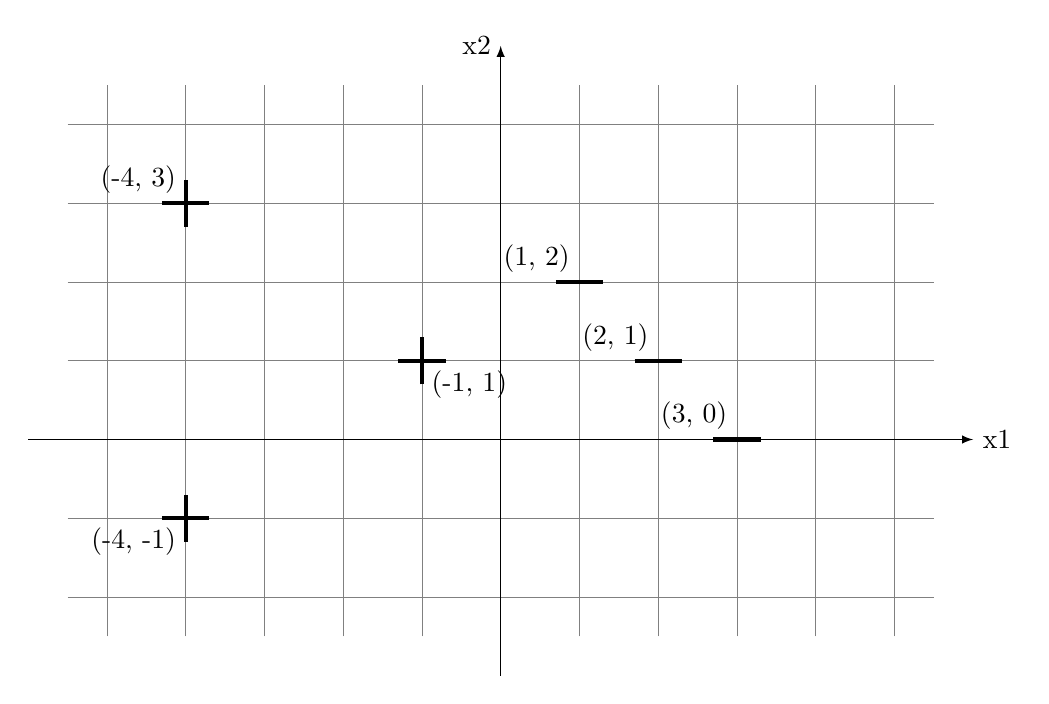
\begin{tikzpicture}
		\tikzstyle {point line} = [line width=0.15em]
		\tikzstyle {margin} = [dashed]
														
		\draw[step=1.0, gray, very thin] (-5.5, -2.5) grid (5.5, 4.5);
																		    
		\draw[-latex] (-6,0) -- (6,0) node[right]{x1};
		\draw[-latex] (0,-3) -- (0,5) node[left]{x2};	
																
		\draw[point line] (-1.3, 1) -- (-0.7, 1);	
		\draw[point line] (-1, 0.7) -- (-1, 1.3);
		\draw (-1, 1) node [below right] {(-1, 1)};    	
														
		\draw[point line] (-4.3, -1) -- (-3.7, -1);	
		\draw[point line] (-4, -1.3) -- (-4, -0.7);	
		\draw (-4, -1) node [below left] {(-4, -1)};   
														
		\draw[point line] (-4.3, 3) -- (-3.7, 3);	
		\draw[point line] (-4, 2.7) -- (-4, 3.3);	
		\draw (-4, 3) node [above left] {(-4, 3)};   
														
		\draw[point line] (1.7, 1) -- (2.3, 1);		
		\draw (2, 1) node [above left] {(2, 1)}; 
						
		\draw[point line] (2.7, 0) -- (3.3, 0);		
		\draw (3, 0) node [above left] {(3, 0)};
						
		\draw[point line] (0.7, 2) -- (1.3, 2);		
		\draw (1, 2) node [above left] {(1, 2)};				  
															   		
	\end{tikzpicture}
\end{figure}

The means for the respective classes are,

\begin{align*}
	\boldsymbol{m_{+}} & = \begin{pmatrix} 
	-3 \\
	1 
	\end{pmatrix} \\
	\boldsymbol{m_{-}} & = \begin{pmatrix} 
	2 \\
	1 
	\end{pmatrix}    
\end{align*}

Now, the between-class scatter matrix is calculated as follows,

\begin{align*}
	\boldsymbol{S_B} & = (\boldsymbol{m_{+}} - \boldsymbol{m_{-}})(\boldsymbol{m_{+}} - \boldsymbol{m_{-}})^T \\ 
	                 & = \begin{pmatrix}                                                                      
	-5 \\
	0 
	\end{pmatrix} \begin{pmatrix}
	-5               & 0                                                                                      
	\end{pmatrix} \\
	                 & = \begin{pmatrix}                                                                      
	25               & 0                                                                                      \\
	0                & 0                                                                                      
	\end{pmatrix}         
\end{align*}

And then, the within-class scatter matrix is calculated,

\begin{align*}    
	S_+              & = \sum_{i \in +}(\boldsymbol{x_i} -\boldsymbol{m_+})(\boldsymbol{x_i} -\boldsymbol{m_+})^T \\
	                 & = \begin{pmatrix}                                                                          
	2 \\
	0
	\end{pmatrix} \begin{pmatrix}
	2                & 0                                                                                          
	\end{pmatrix} + \begin{pmatrix}
	-1 \\
	2
	\end{pmatrix} \begin{pmatrix}
	-1               & 2                                                                                          
	\end{pmatrix} + \begin{pmatrix}
	-1 \\
	-2
	\end{pmatrix} \begin{pmatrix}
	-1               & -2                                                                                         
	\end{pmatrix}  \\
	                 & = \begin{pmatrix}                                                                          
	6                & 0                                                                                          \\
	0                & 8                                                                                          
	\end{pmatrix} \\
	S_-              & = \sum_{i \in -}(\boldsymbol{x_i} -\boldsymbol{m_-})(\boldsymbol{x_i} -\boldsymbol{m_-})^T \\
	                 & = \begin{pmatrix}                                                                          
	0 \\
	0
	\end{pmatrix} \begin{pmatrix}
	0                & 0                                                                                          
	\end{pmatrix} + \begin{pmatrix}
	-1 \\
	1
	\end{pmatrix} \begin{pmatrix}
	-1               & 1                                                                                          
	\end{pmatrix} + \begin{pmatrix}
	1 \\
	-1
	\end{pmatrix} \begin{pmatrix}
	1                & -1                                                                                         
	\end{pmatrix}  \\
	                 & = \begin{pmatrix}                                                                          
	2                & -2                                                                                         \\
	-2               & 2                                                                                          
	\end{pmatrix} \\
	\boldsymbol{S_W} & = \boldsymbol{S_+} + \boldsymbol{S_-}                                                      \\
	                 & = \begin{pmatrix}                                                                          
	8                & -2                                                                                         \\
	-2               & 10                                                                                         
	\end{pmatrix}
\end{align*}

The eigenvalue problem is formulated as,

\begin{align*}
	\boldsymbol{S_B}\boldsymbol{w} = \lambda \boldsymbol{S_W}\boldsymbol{w} 
\end{align*}

Equating the determinant of $\boldsymbol{S_B} - \lambda \boldsymbol{S_W}$ to zero,

\begin{align*}
	\begin{vmatrix}
	25-8\lambda   & 2\lambda   \\
	2\lambda      & -10\lambda 
	\end{vmatrix} & = 0        \\
	\lambda = \frac{125}{38}
\end{align*}

The corresponding eigenvector amounts to $\frac{1}{\sqrt{26}}\begin{pmatrix}
5 \\
1
\end{pmatrix}$ which is the direction of projection. The below plot helps to visualize how this projection direction divides the two classes.

\FloatBarrier\clearpage
\begin{figure}[htbp]
	\centering
	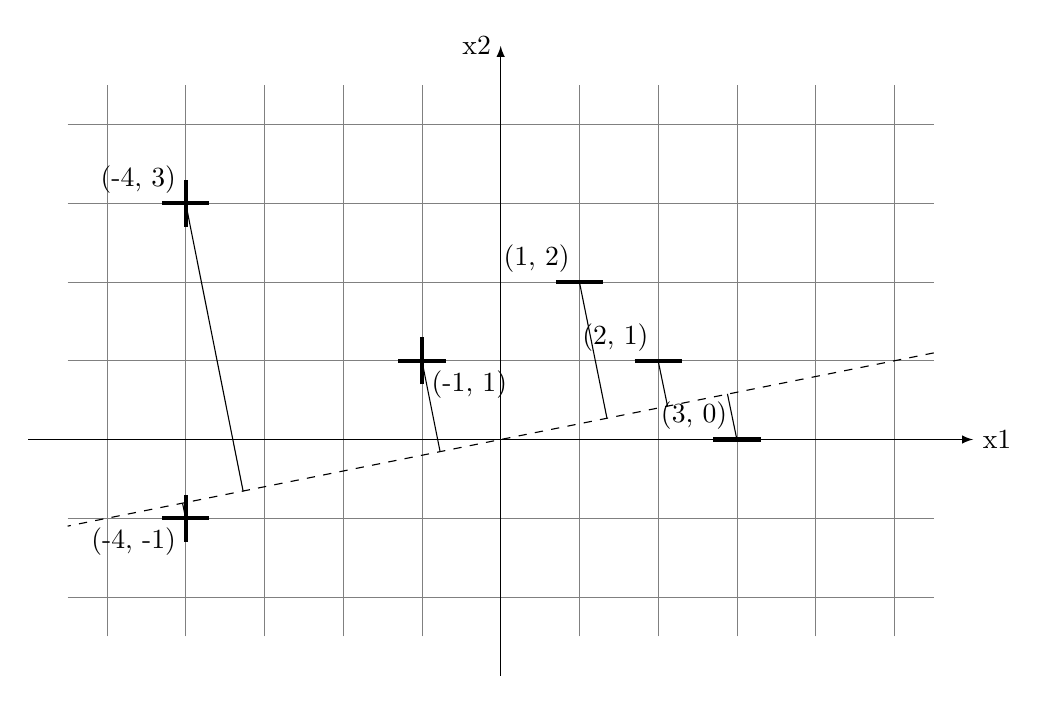
\begin{tikzpicture}
		\tikzstyle {point line} = [line width=0.15em]
		\tikzstyle {margin} = [dashed]
														
		\draw[step=1.0, gray, very thin] (-5.5, -2.5) grid (5.5, 4.5);
																		    
		\draw[-latex] (-6,0) -- (6,0) node[right]{x1};
		\draw[-latex] (0,-3) -- (0,5) node[left]{x2};	
																
		\draw[point line] (-1.3, 1) -- (-0.7, 1);	
		\draw[point line] (-1, 0.7) -- (-1, 1.3);
		\draw (-1, 1) node [below right] {(-1, 1)};    	
														
		\draw[point line] (-4.3, -1) -- (-3.7, -1);	
		\draw[point line] (-4, -1.3) -- (-4, -0.7);	
		\draw (-4, -1) node [below left] {(-4, -1)};   
														
		\draw[point line] (-4.3, 3) -- (-3.7, 3);	
		\draw[point line] (-4, 2.7) -- (-4, 3.3);	
		\draw (-4, 3) node [above left] {(-4, 3)};   
														
		\draw[point line] (1.7, 1) -- (2.3, 1);		
		\draw (2, 1) node [above left] {(2, 1)}; 
						
		\draw[point line] (2.7, 0) -- (3.3, 0);		
		\draw (3, 0) node [above left] {(3, 0)};
						
		\draw[point line] (0.7, 2) -- (1.3, 2);		
		\draw (1, 2) node [above left] {(1, 2)};
						
		\draw[dashed] (5.5, 1.1) -- (-5.5, -1.1);	
		\draw[thin] (-4, -1) -- (-4.04, -0.81);	
		\draw[thin] (-1, 1) -- (-0.77, -0.15);
		\draw[thin] (-4, 3) -- (-3.27, -0.66);
					    	
		\draw[thin] (1, 2) -- (1.35, 0.27);
		\draw[thin] (2, 1) -- (2.12, 0.42);	    	    
		\draw[thin] (3, 0) -- (2.88, 0.58);	    
															   		
	\end{tikzpicture}
\end{figure}

\section{Multi-Class Case}

In two class case dimensionality was reduced to 1. In $K$ class case, it is reduced to $K-1$. Hence, instead of finding an optimal $d$-dimensional vector $\boldsymbol{w}$ in the two class case, a matrix of $K-1$ $d$-dimensional vectors $\boldsymbol{W}^T = \begin{pmatrix}
\boldsymbol{w_1}^T \\
\boldsymbol{w_1}^T \\
\vdots \\
\boldsymbol{w_{K-1}}^T \\        
\end{pmatrix}$ must be found. The projection is defined as $\boldsymbol{y}=\boldsymbol{W}^T\boldsymbol{x}$ where $\boldsymbol{y}$ is a $K-1$ dimensional vector as expected.

The generalization for within-class matrix is as follows,

\begin{align*}
	\boldsymbol{S_W} = \sum_{k=1}^K \sum_{i \in C_k} (\boldsymbol{x_i} - \boldsymbol{m_k})(\boldsymbol{x_i} - \boldsymbol{m_k})^T 
\end{align*}
 
For generalizing between-class matrix, consider the total scatter matrix $\boldsymbol{S_T}$ as follows,

\begin{align*}
	\boldsymbol{S_T} & = \sum_{i=1}^N (\boldsymbol{x_i} - \boldsymbol{m})(\boldsymbol{x_i} - \boldsymbol{m})^T                                                                                                                               \\
	                 & = \sum_{k=1}^K \sum_{i \in C_k} (\boldsymbol{x_i} - \boldsymbol{m})(\boldsymbol{x_i} - \boldsymbol{m})^T                                                                                                              \\
	                 & = \sum_{k=1}^K \sum_{i \in C_k} (\boldsymbol{x_i} - \boldsymbol{m_k} + \boldsymbol{m_k} - \boldsymbol{m})(\boldsymbol{x_i} - \boldsymbol{m_k} + \boldsymbol{m_k} - \boldsymbol{m})^T                                  \\
	                 & = \sum_{k=1}^K \sum_{i \in C_k} (\boldsymbol{x_i} - \boldsymbol{m_k})(\boldsymbol{x_i} - \boldsymbol{m_k})^T + \sum_{k=1}^K \sum_{i \in C_k} (\boldsymbol{m_k} - \boldsymbol{m})(\boldsymbol{m_k} - \boldsymbol{m})^T \\
	                 & = \boldsymbol{S_W} + \sum_{k=1}^K N_k(\boldsymbol{m_k} - \boldsymbol{m})(\boldsymbol{m_k} - \boldsymbol{m})^T                                                                                                         \\
	                 & = \boldsymbol{S_W} + \boldsymbol{S_B}                                                                                                                                                                                 
\end{align*} 

The maximization problem is then generalized as follows,

\begin{align*}
	J(\boldsymbol{W}) = \frac{det(\boldsymbol{W}^T \boldsymbol{S_B} \boldsymbol{W})}{det(\boldsymbol{W}^T \boldsymbol{S_W} \boldsymbol{W})} 
\end{align*}

The solution to find the matrix $\boldsymbol{W}$ is to find the largest $K-1$ eigenvalues of the following equation and arrange the corresponding eigenvectors in a matrix. 

\begin{align*}
	\boldsymbol{S_B}\boldsymbol{w} = \lambda \boldsymbol{S_W}\boldsymbol{w} 
\end{align*}    

Additionally, there are no more than $K-1$ non-zero eigenvectors to the above 
equation due to the redundancy of the matrix $\boldsymbol{S_B}$ as was seen in the two class case.
 
\end{document}
